%!TEX root = ../main.tex

\chapter{Introduction}
\label{chp:intro}

In this chapter, we will draw a background for our study topic. First, we will have a brief overview of Machine Learning and some of its sub-fields and applications. We will present some further details about Deep Learning and give a blueprint for the training procedure of the Deep Learning models. Later, we will look closely at the purpose and sub-fields of Natural Language Processing, and the importance of word embeddings in particular. Building on this, in Chapter-\ref{chp:stateOfArt}, we will see some of the state-of-the-art embedding techniques, and how they differ from one another.


\section{Background: Machine Learning}

%\subsection{What is Machine Learning?}

\ac{ML} is an \ac{AI} sub-field focused on developing algorithms and statistical models that enable computer systems to learn from data, to gain the ability to make predictions or decisions, without the need for explicit programming of rules. These predictions or decisions can be described as a wide range of tasks, from the detection of a range of objects in the input images \cite{maskrcnn}, to estimating future stock prices based on a diverse set of variables \cite{stockmarket}.

Machine learning algorithms use mathematical and computational techniques to learn from data. These algorithms learn by tuning their parameters based on the training data to improve their performance as learning progresses. The direction in which parameters should be changed is determined by the target functions designated by the system designers. A machine learning model can operate on data in many formats, such as text, image, audio, strings of numbers, combinations of these, and many others. Unlike traditional software development paradigms, where rules and logic are programmed explicitly, machine learning systems derive their rules and logic from data. This enables them to carry out complex tasks for which it is difficult to clearly define the rules.

\subsection{Machine Learning: Use of data in learning}

\ac{ML} can be broken down into three main approaches, in terms of the use of the data. All \ac{ML}-related tasks can be said to employ one of the following paradigms in terms of the role of data in learning: \textbf{Supervised Learning}, \textbf{Unsupervised Learning}, or \textbf{Reinforcement Learning}. Even though it is possible to draw further branches from these paradigms, for now, this level of detail will be sufficient.

A \textbf{supervised} learning system learns under the assumption that there is a ground truth and the goal is to approximate it by tuning the internal parameters. This paradigm can be employed when the objective is to learn from a given set of decisions and imitate their thought process on new data later on. This is applicable for scenarios such as when the goal is to develop a computed tomography analyzer and there is a set of analyzed CT images available \cite{strokedet}, or if the goal is to create a system that can detect sarcasm in the text when a dataset of annotated text for this purpose is present \cite{sarcasmdet}.

\textbf{Unsupervised} learning, on the other hand, is suitable for making decisions or predictions on data, without the need to learn certain rules from a supervisor beforehand. Even though it is usually ideal to have a teacher to correct the mistakes of the system, eliminating the need for it can relieve the designers from the necessity of collecting and annotating a proper dataset. 

\textbf{Reinforcement} learning is a more distinct paradigm than the other two. It is rather about trial and error. The learning task is modeled as the process of learning a \textit{policy} that maps each possible \textit{state configuration} to \textit{actions}, in order to maximize a \textit{cumulative reward}. The learning agent is exposed to the \textit{environment} and able to manipulate it for a given number of \textit{episodes}, and the \textit{observations} made in progress are useful for the learning task. This is useful for tasks like motion learning of robotic arm manipulators \cite{robotRL}, or the development of a model that can play Atari games \cite{atariRL}, and many more.

\subsection{Deep Learning}

\ac{DL} is a sub-field of \ac{ML} that encompasses a class of \ac{ANN}s characterized by their depth. The main goal of deep learning is to automatically learn hierarchical representations of data.

The core of deep learning is \ac{ANN}s, specifically \ac{DNN}s, which consist of interconnected nodes, or \textit{neurons}, organized in \textit{layers}. These neurons are the building blocks of an \ac{ANN} and are responsible for calculations. Their input is provided by the neurons in the previous layer, and their output is the input of the neurons in the next layer. These input and output connections between neurons are associated with certain coefficients, called \textit{weights}. Neurons apply nonlinear operations using \textit{activation functions}, and this non-linearity is the factor that enables neural networks to solve more complex problems.

Generally, a \ac{DNN} consists of an input layer, one or more hidden layers, and an output layer. The input layer is where the network receives data, and the number of neurons depends on the format and shape of the input. Hidden layers, stacked between the input and output layers, are responsible for converting input data into increasingly more abstract representations. The output layer produces final predictions based on the representations learned in the previous layers. The architecture and number of nodes in this layer depend on the task, such as classification, regression, or generation. A simple feedforward neural network architecture is given in Figure \ref{fig:feedforward}.


\begin{figure}[ht]
    \begin{minipage}{\textwidth}
        \centering
        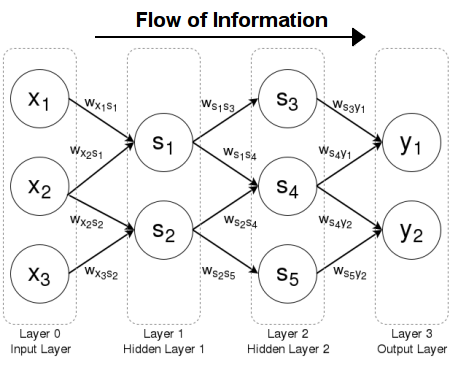
\includegraphics[width=0.5\textwidth]{img/feedforward_NN.png}
        \caption[A simple deep feedforward neural network with two hidden layers.]{A simple deep feedforward neural network with two hidden layers.\footnote{Source: \url{https://brilliant.org/wiki/feedforward-neural-networks/}}}
        \label{fig:feedforward}
    \end{minipage}
\end{figure}

Deep learning models are trained using large datasets and optimization techniques to adjust the weights and biases of connections between neurons. The complexity of the network is decided based on several factors, such as the complexity of the task, the size and proportion of training data, and the desired performance. This training process aims to minimize the error or loss function by effectively tuning the model's parameters to make accurate predictions on previously unseen data. Depending on the complexity of the tasks or the availability of certain types of samples in the data, training of deep models can get quite data-hungry.

The general architecture mentioned is valid for standard \ac{FNN}s, but many different architectures exist for different tasks and needs. Some of the most popular are \ac{CNN}, \ac{RNN}, \ac{GNN}, and \ac{LSTM}. For example, \ac{CNN}s are very useful for processing matrix-formatted input data, and \ac{RNN}s are designed for temporal data where previous input history is useful for decision-making.

\begin{figure}[ht]
    \begin{minipage}{\textwidth}
        \centering
        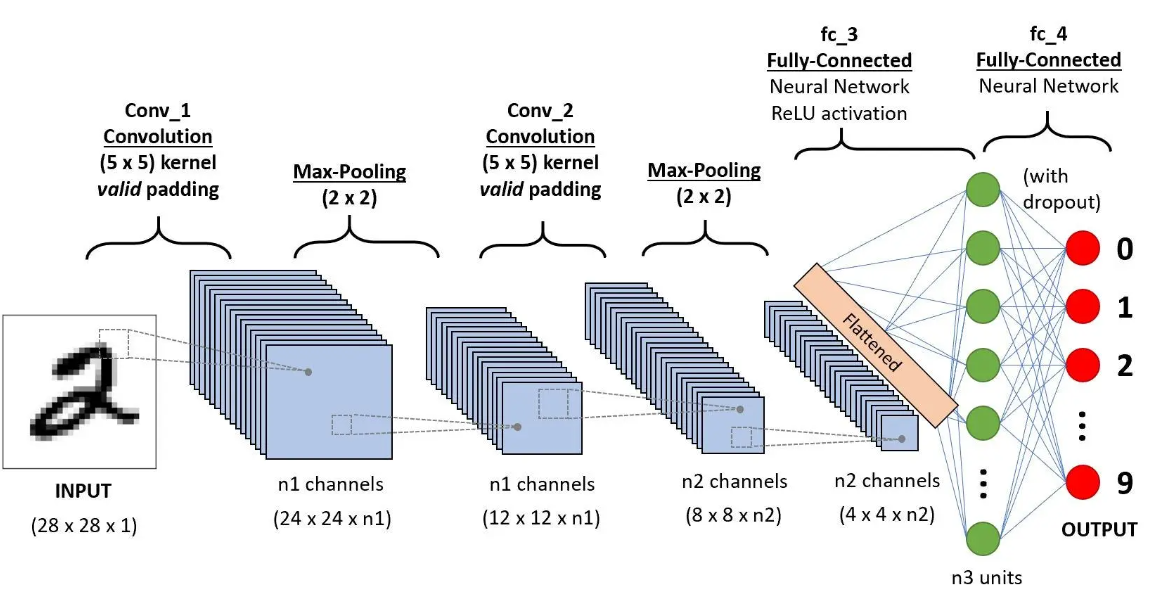
\includegraphics[width=0.8\textwidth]{img/cnn.png}
        \caption[A Convolutional Neural Network architecture for handwritten digit recognition.]{A Convolutional Neural Network architecture for handwritten digit recognition.\footnote{Source: \cite{CNNimg}}}
        \label{fig:cnn}
    \end{minipage}
\end{figure}

Deep learning models have achieved remarkable success in a variety of fields and provided solutions for a range of problems that were previously thought to be not solvable with computers. This is achieved thanks to the automatic discovery of complex patterns and representations from raw data.

\subsection{Training of a deep learning model}

Now we will have a closer look at the training procedure of \ac{DL} models. This way we will have an intuition about the training procedure of our word embedding model, which will be described later on.

The training procedure is essentially a systematic search for the optimal configuration of parameters. The optimality of a configuration is indicated by a target or a loss function. The optimal configuration is the configuration that maximizes the target function, or that minimizes the loss function. We will use the loss function in our descriptions. Therefore, the goal of the training is formulated as an optimization problem of the loss function. Building on this, the definition of the optimal parameter configuration \(\theta^*\) is:

\[ \theta^* = \arg\min_\theta \left[ \mathbb{E}[L(\hat{Y}, Y)] \right] \]

\noindent
where \(Y\) is the vector of the true target values, \(\hat{Y}\) is the model's predictions made with the configuration \(\theta\) for the input data, \(L\) is a function that measures the discrepancy between the model's predictions and the true labels.

The above definition is more accurate for a supervised learning setting, but loss-based optimization is also applicable to an unsupervised learning system. In this case, the loss is calculated only using the network predictions. We can generalize the definition as:

\[ \theta^* = \arg\min_\theta \left[ \mathbb{E}[L(Y)] \right] \]

In real-life scenarios, finding this optimal configuration is not always possible, therefore we usually settle with "close enough". We mentioned that this procedure is systematic, meaning it operates on a pipeline with a designated set of steps. Depending on the task, these steps do differ, however, we will try to list the ones that are somewhat common in all \ac{DL}-related tasks.

\textbf{Data Collection:} For the learning of a \ac{DL} model, the first thing to do is to create a dataset. With the increasing interest in \ac{AI} and \ac{DL}, this step is often omitted, since there is usually a dataset suitable for the majority of the tasks available online. When this is not the case, the creation of a dataset includes gathering data samples that are in the same format as the samples that the model will make predictions on after the training. These samples should be organized in a usable format, and if needed, missing and mistaken values should be handled. This procedure is often called \textit{data cleaning}. Afterward, if needed, the samples should go through steps of preprocessing before the training. These steps can be designed to prepare the samples for the training procedure or increase the training efficiency. For example, we needed to first tokenize our corpus, and it was needed for creating training batches. On the other hand, we also removed stop-words, but this was for capturing more contextual information. In the majority of the applications when the number of training samples is sufficient, the preprocessing also involves splitting the dataset into training, test, and validation sets. This is needed for training the model, monitoring its progress, and fairly evaluating its final performance by using a single dataset.

\textbf{Model Design:} The next thing is to design the model architecture. For \ac{ANN}s, this means deciding the number and types of layers, the number of neurons in each layer, and the activation functions. These are decided based on the type and the complexity of the task, the number of training samples available, and the shape of the input data. Once this is done, the weights of neuron connections are initialized. The most natural idea is the random initialization, but considering that this can greatly impact the training, this is yet another thing that the designer should be mindful of.

\textbf{Loss Function:} Loss function is one of the most important factors of the training procedure. The goal of training is modeled as the minimization of the loss function. Therefore, it is very important that the loss function accurately represents the goal of training. There are loss functions commonly used for different tasks, for example for regression, \ac{MSE} Loss is a common choice, or for binary classification \ac{CE} loss is commonly used. For the unsupervised setting, there are popular loss options such as \textit{inertia} for clustering tasks and \textit{autoencoder loss} for dimensionality reduction. For more specific tasks, the designer must design a custom loss function, representing the margin between the model's predictions and the true values.

\textbf{Optimizer:} The learning procedure is essentially iteratively updating the weights and bias of the network given the current loss. Updating these weights according to the direction and value indicated by the loss function is done by using an optimizer. The optimizer iteratively optimizes the parameters of the network using gradients. This gradient-based optimization of parameters in a single iteration can be formulated as:

\[
\theta_{k+1} = \theta_k - \alpha \nabla L
\]
\noindent
where \(\theta_k\) is the parameter vector at iteration $k$, \(\theta_{k+1}\) is the parameter vector at iteration $k+1$, \(\alpha\) is the learning rate (see Hyperparameters below), and \(\nabla L\) is the gradient of the loss with respect to the network parameters.

Different optimizers can do this operation in different ways, some update all parameters at once, while others work with batches (small subsets of data). Some make all updates according to the same learning rate, but some automatically find the appropriate learning rate for different parameters. Some of the most common optimizers are \ac{SGD}, Adam, and RMSprop.

\textbf{Hyperparameters:} Hyperparameters are parameters that shape the training procedure. They are not learned, in other words, the values assigned to them at the beginning of the training do not change throughout the training. There are many hyperparameters, but some of the most common are the number of epochs, batch size, and learning rate. The number of epochs is the number of times the entire training data passes through the entire network. Choosing the wrong epoch number might result in \textit{overfitting} or \textit{underfitting}. Batch size is the size of the groups to be used in the parameter update procedure. The wrong batch size will cause training to be too slow or introduce too much noise in learning. The learning rate is the step size of the parameter updates. A not-so-ideal learning rate can slow down the training or cause it not to converge to optimal values. It is common practice to run the training several times with different hyperparameter configurations and compare the results, as these have a direct impact on the final performance of the model and the ideal configuration is usually not very straightforward.

\textbf{Training Loop:} Once the training starts, we iterate over the training data in mini-batches. A mini-batch is a small subset of data. Working with mini-batches is a good balance between training with the entire dataset at once and going sample by sample. The motivation for this approach is to speed up the training by also reducing memory usage. 
At each step, for each mini-batch, we follow four steps.

\begin{enumerate}
  \item \textbf{Forward Pass:} Model makes predictions given the training data as the input.
  \item \textbf{Loss Computation:} Given the model predictions (and the true labels, if supervised), calculation of the discrepancy. 
  \item \textbf{Backpropagation:} Computation of the gradient of the loss with respect to the parameters of the network.
  \item \textbf{Parameter Update:} Based on the computed gradients, the optimizer adjusts model parameters in the direction that minimizes loss. The size of this adjustment is based on the gradient and the learning rate.
\end{enumerate}

These four steps are applied for the number of epochs for the entire training set. A good choice of the number of epochs yields a satisfactory training accuracy, but not by overfitting.
It is usually a good idea to monitor system performance throughout the training. This will be useful for fine-tuning the parameters and detecting overfitting early on. This can be done using a validation set, by monitoring the validation loss calculated using the labels of validation data and the model's predictions on them. It is very important to not include the validation samples in the training set. Once the training is completed, these results can be visualized to give a better perspective on the effectiveness of the training algorithm.

\textbf{Evaluation:} Once the training is completed, the model's performance is evaluated on unseen test samples. These samples can be taken from the same dataset or some other, but the main thing to pay attention to is that this data should not be seen by the model during the training. Based on the loss calculated with this test data, one can have a better idea about the generalization capability of the model. Common practice is to use metrics like \textit{recall}, \textit{precision}, and \textit{f1-score} when applicable.




\section{Background: Natural Language Processing}

Understanding \ac{NLP} and its significance is important as it underpins the motivation for exploring static word embeddings in this dissertation.

%\subsection{What is Natural Language Processing?}

\ac{NLP}, a sub-field of \ac{AI}, is dedicated to the medium of natural language, used in the human interactions. It enables machines to read, process, and derive meaning from text-formatted data. As the amount of text data gets larger, it contains more useful information, but it also gets more challenging to extract it. The emergence of \ac{NLP} was driven by the need for automated processing of data in text format, which is rapidly growing in size. 

\ac{NLP} made it possible to use the natural language for communication between humans and computer programs.  However, the natural languages used in human lives have a very complex nature, which makes it challenging to model and interpret them by our machines for mathematical calculations. Therefore, it all begins with the recognition that human language is large, inherently complex, and characterized by nuances, idiomatic expressions, and context-dependent senses.

\ac{NLP} is an interdisciplinary field that intersects with linguistics, computer science, artificial intelligence, statistics, and cognitive psychology. Its multifaceted nature allows researchers to approach the challenges using the knowledge collected in a range of research fields, to tackle a wide array of linguistic phenomena, ranging from syntax and semantics to pragmatics and discourse analysis.


\subsection{Why is Natural Language Processing Challenging?}
Despite its progress, \ac{NLP} faces numerous challenges due to the complexity of the natural languages. Some of these challenges are:

\begin{itemize}
\item Language interpretation is ambiguous.
\item Need to deal with a wide set of languages and their different dialects. Different languages not only have different words and phrases but also sometimes they differ greatly in their syntactics.
\item Even though it is usually straightforward for humans to recognize sarcasm, irony, and humor, it can be very tricky for computers.
\item Need to adapt to always-changing linguistic trends and cultural shifts. New trends might reduce the use of a common word, or introduce new words, new phrases, and different uses of the existing words.
\end{itemize}

Most of these challenges stem from the properties of natural languages. Such as:

\begin{itemize}
\item \textbf{Ambiguity}: It emerges in different scales. Sounds can have different transcriptions, words can have different senses and sentences can have different interpretations. 
\item \textbf{Compositionality}: The meaning of multi-element linguistic expressions is given by some function of the meaning of lower-level units and the way they are syntactically combined together.
\item \textbf{Recursion}: A language is based on some grammar. The rules of grammar can iterate on words to generate an infinite number of compositions, each with its specific meaning.
\item \textbf{Hidden Structure}: The language is believed to have a hidden structure, as any local change in a sentence can potentially disrupt the interpretation of the entire expression.
\end{itemize}

\subsection{Applications of NLP}

Thanks to the advancements in machine learning, \ac{NLP} studies have spread over a very wide scope due to its vast array of real-world applications, including:

\begin{itemize}

\item \textbf{Machine translation}, overcoming the language barriers for information exchange.
\item \textbf{Sentiment analysis}, revealing public sentiment towards products, services, artistic creations, political figures, ideas, events, and many more.
\item \textbf{Fake news detection}, protecting public opinion from misleading statements.
\item \textbf{Chatbots and virtual assistants}, enabling human-like interactions with machines.
\item \textbf{Question Answering}, automatically learning from existing data for more efficient learning from it by humans.
\item \textbf{Information retrieval}, for information extraction from unstructured and possibly large text formatted data.
\item \textbf{Text summarization}, condensing lengthy texts into concise summaries.
\item \textbf{Speech recognition}, converting speech into text.

\end{itemize}

These and many other applications of \ac{NLP} are beneficial for commercial use, but also handy in our personal lives. For commercial use, they enabled companies to optimize their operations and engage better with their customers, increasing their revenues in the scale of millions in some instances \cite{comm-nlp}. They also come in handy in many forms for us in our daily lives, such as auto-complete-supported digital keyboards, language model-supported smart search engines \footnote{As of today, the most known product: \url{https://www.bing.com}}, and smart home assistants.


\subsection{Background: Word embeddings}

Representation of words in a human mind is not applicable to today's machine learning algorithms, therefore we need another way of representing them. For this purpose, we use word embeddings, an appropriate representation of words that can be comprehended by machine learning algorithms. Word embeddings are the building blocks of \ac{NLP} applications. Essentially, an embedding of a word is a vector in a high-dimensional vector space, containing the semantic and syntactic characteristics of that word. Embeddings bridge the gap between the discrete nature of words and the continuous mathematical spaces. Representing a word as a high-dimension vector can implicitly encode rich linguistic information. This is a crucial property for almost all \ac{NLP} tasks, as it enables machines to learn and store not only the meaning of words but also the contextual associations between them. 

When we say word embeddings, usually we mean either one of two kinds of them. We will briefly introduce both, but for the rest of this dissertation, we will use the terms "Word Embeddings" and "Static Word Embeddings" interchangeably. 

\subsubsection{Static word embeddings}

Static word embeddings (also known as \textbf{pre-trained word embeddings}) are vector representations of words generated by learning from a large, static corpus. The name of these models suggests the fact that these embeddings are computed before the downstream \ac{NLP} task and cannot be modified once the learning phase is completed. Usually, static embeddings are computed with matrix factorization or shallow neural networks.

When used, the word embeddings are stored and accessed just like using a dictionary. Every \textbf{type} in the corpus corresponds to one unique vector and it is the same regardless of the context in which the word occurs. From this, it is easy to see that if a word is not present in the training corpus, the embedding model will not generate an embedding for it, and one needs to tackle this issue during the downstream task appropriately.

Static word embeddings are mostly based on the \textit{distributional hypothesis}, which says that words with similar meanings are likely to occur in similar contexts. In other words, within the corpus, words that are surrounded by similar words, or frequently co-occur with each other, should have similar meanings. Learning from a fixed corpus, these embeddings are designed to approximate the statistical patterns of word co-occurrence. For this approximation, different algorithms rely on different statistical measures, such as co-occurrence frequencies or \ac{PMI}, to determine the contextual relationships of words.

Even though they are more straightforward to train and easier to use, static embeddings usually fail to capture more fine-grained contextual characteristics of the words. A static word embedding model can be perfectly able to list the most similar and related words to a given word, but distinguishing different word senses is a difficult challenge even for the most popular static embedding models.

\subsubsection{Dynamic word embeddings}

Dynamic word embeddings (also known as \textbf{contextual word embeddings}) are context-aware word representations. These embeddings are generated dynamically for each \textbf{token} in the corpus based on the surrounding words in a given context. They are commonly trained using artificial neural networks (for example, \ac{ELMo} architecture uses a bi-directional \ac{LSTM} model \cite{elmo}), and transformers (\ac{BERT} is based on a multi-layer bidirectional transformer encoder \cite{bert}).

Dynamic word embeddings are generated by taking into account the neighboring words to a target word in a given context. They succeed in word sense disambiguation and context-dependent meanings.

Dynamic embeddings are closely related to the task of language modeling. Many language models rely on dynamic word embeddings to capture contextual characteristics and relationships of words. After the embeddings are learned from a large corpus, the vectors later can be conveniently fine-tuned in the pre-training of downstream \ac{NLP} task.









